\chapter[Resultados]{Resultados}

\section{Solução Desenvolvida}

\subsection{Tecnologias e ferramentas utilizadas}

Para a construção da proposta de solução final foram utilizadas algumas ferramentas, tecnologias e bibliotecas ao longo do processo de desenvolvimento. A seguir estas estão elencadas junto com a motivação de sua utilização dentro da solução:

    \begin{quote}
    \begin{itemize}
        \item ReactJS: Biblioteca javascript utilizada para criar a interface dos diferentes módulos da solução.
        \item Material UI: Biblioteca de componentes ReactJS para um desenvolvimento ágil e fácil, sendo utilizado para criar um visual mais agradável para a aplicação.
        \item Web3.Js: Coleção de bibliotecas que possibilitam a interação com nós ethereum remotos, utilizando conexões HTTP ou ICP. Possibilitando assim que os clientes possam se comunicar com o contrato inteligente desenvolvido.
        \item Metamask: Extensão de navegador para acesso a aplicativos distribuídos(Dapps), onde a mesma injeta a API Ethereum do Web3 no contexto javascript dos sites. Também permite que os usuários criem e gerenciem suas próprias identidades e transações, trazendo uma interface segura para revisar transações antes de aceitá-las ou rejeitá-las.
        \item Docker e Docker-compose: Containers utilizados para facilitar o gerenciamento de dependências da aplicação assim como orquestrar facilmente os ambientes de desenvolvimento e produção das mesmas.
        \item TESTNET Ropsten (ETH): Rede ethereum que executa o mesmo protocolo que o Ethereum(main net) e é usada para fins de teste. O contrato inteligente da solução está registrado nesta e rede e todas as transações ocorrem em interações dentro dela.
        \item Ropsten Ethereum Faucet: Ferramenta utilizada para obter ethers gratuitos da rede de testes Ropstas para as contas utilizadas na solução;
        \item Digital Ocean: Serviço de hospedagem utilizado para hospedar os módulos(Dapps) desenvolvidos em servidores linux, para que as aplicações possam ser acessadas sem a necessidade de executá-las localmente.
        \item Solidity: Linguagem de programação de alto nível por meio da qual é possível criar aplicações descentralizadas, em especial os smart contracts, na Ethereum. 
        \item Truffle: Um ambiente de desenvolvimento, framework de testes e pipeline de ativos para blockchains usando a Ethereum Virtual Machine (EVM). Tendo sido utilizado principalmente na fase inicial de construção do contrato inteligente, possibilitando o desenvolvimento do mesmo mais rapidamente.
        \item Ganache: Blockchain Ethereum pessoal utilizado executar testes, executar comandos e inspecionar o estado enquanto controla como a cadeia de blocos opera localmente.
    \end{itemize}
    \end{quote}
        
\subsection{Arquitetura da Solução}

A solução foi desenvolvida seguindo uma arquitetura cliente-servidor, representada na figura \ref{fig:dapp_arquitetura_solucao}. A parte do cliente nesta solução é composto pelas aplicações descentralizadas desenvolvidas(módulos), onde um Dapp corresponde ao sistema utilizado pelas autoridades de trânsito e o outro Dapp sendo o sistema de acesso dos motoristas. Já o servidor da solução corresponde a rede ethereum onde o \verb|deploy| do contrato inteligente foi feito e as transações são validadas pelos nós mineradores da rede, representado na figura \ref{fig:dapp_rede_ethereum}.

    \begin{figure}[h]
         \centering
         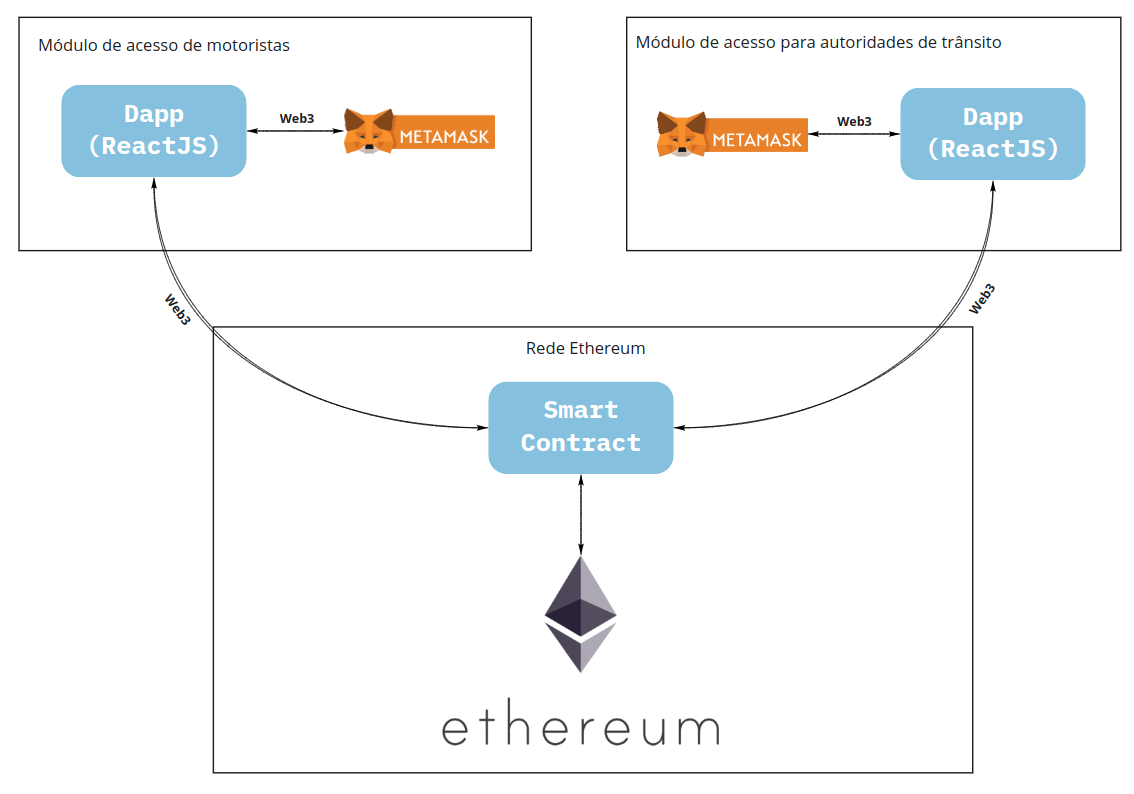
\includegraphics[scale=0.35]{figuras/capitulo_5/arquitetura_solucao.png}
         \caption{Representação da interação entre os módulos da solução - Imagem própria.}
         \label{fig:dapp_arquitetura_solucao}
    \end{figure}
    
    \begin{figure}[h]
         \centering
         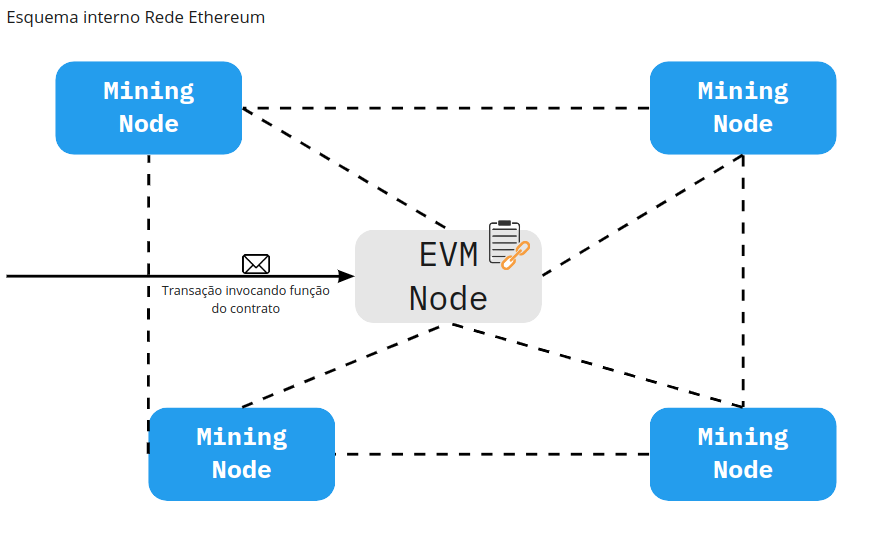
\includegraphics[scale=0.4]{figuras/capitulo_5/esquema_rede_ethereum.png}
         \caption{Representação da rede Ethereum onde o contrato está na Ethereum Virtual Machine - Imagem própria.}
         \label{fig:dapp_rede_ethereum}
    \end{figure}

\subsection{Funcionalidades}